\begin{frame}{Μετά το \texttt{sm2} τι;}


  \definecolor{g}{RGB}{0 150 0}
  \definecolor{r}{RGB}{180 0 0}
  \definecolor{gr}{RGB}{127 127 127}


  \noindent\makebox[\linewidth][c]{%
  \begin{minipage}{\linewidth}
    \begin{figure}\centering
      \resizebox{8cm}{!}{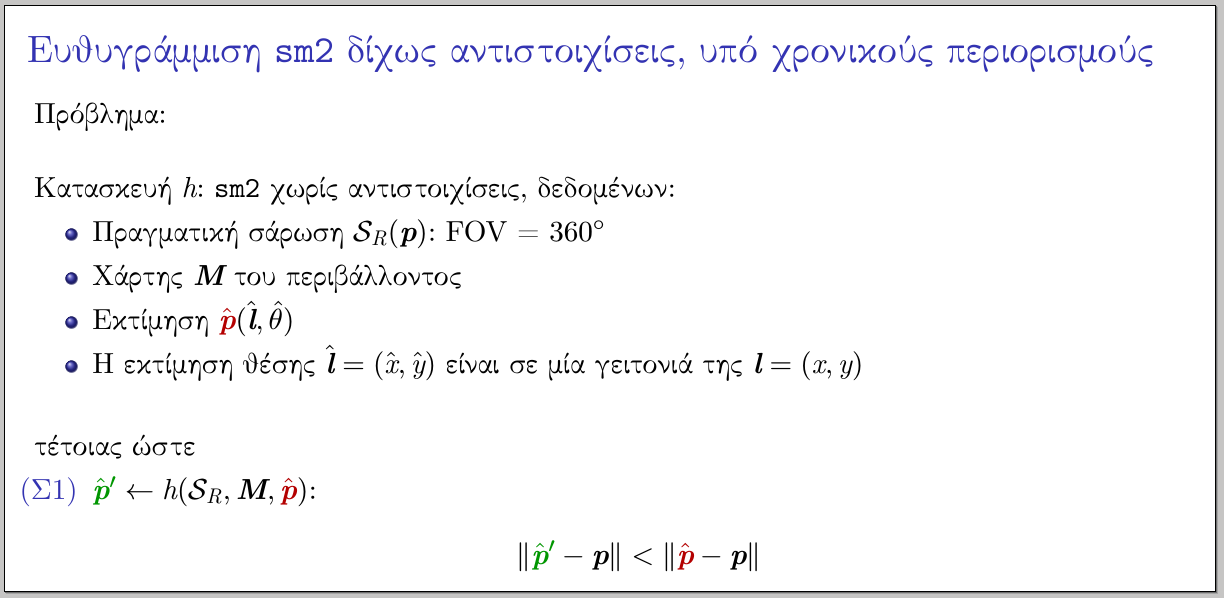
\includegraphics{./figures/slides/ch7/sm2_prob.png}}
      \begin{textblock}{14}(3.35,5.14)
        $\rightarrow \mathcal{S}_R(\bm{p}_1)$
      \end{textblock}
      \begin{textblock}{14}(3.4,5.8)
        $\bigl\} \mathcal{S}_V(\hat{\bm{p}}_0)$
      \end{textblock}
      \begin{textblock}{14}(3.7,6.6)
        $\|\bm{\hat{\bm{l}}}_0-\bm{l}\| < \delta$
      \end{textblock}
    \end{figure}
  \end{minipage}
  }

  \noindent\makebox[\linewidth][c]{%
  \begin{minipage}{\linewidth}
    Εάν $\|\bm{\hat{\bm{l}}}_N-\bm{l}\| \ll \delta$ τότε
    \begin{itemize}
      \item $\|\bm{\hat{\bm{l}}}_{0:N}-\bm{l}\| < \delta$
      \item $\mathcal{S}_V(\hat{\bm{p}}_0) \text{ τοπική προσέγγιση } \bm{M}$ (άρα $\bm{W}$) \vspace{-0.1cm}
      \item[] στη γειτονιά της $\bm{p}, \ \forall \hat{\bm{p}}_i, i = 0,1,\dots,N$
            \makebox(0,0){\put(0,4.7\normalbaselineskip){$\left.\rule{0pt}{2.0\normalbaselineskip}\right\}$
            Εάν $\bm{M} \leftarrow \mathcal{S}_R(\bm{p}_2) \hspace{0.25cm} \Rightarrow h$ λύνει \texttt{sm};
            }}
    \end{itemize}
  \end{minipage}
  }


\note{\footnotesize
Αν ξανακοιτάξουμε το πρόβλημα sm2 όπως το θέσαμε, θα δούμε στα δεδομένα του
προβλήματος μία πραγματική σάρωση, η οποία συλλαμβάνεται από την πραγματική
και άγνωστη στάση του αισθητήρα, και ύστερα το χάρτη του περιβάλλοντος και
μία αρχική εκτίμηση για τη στάση του αισθητήρα. Από αυτά τα δύο δεδομένα
υπολογίζουμε την πρώτη εικονική σάρωση SV. Από τα προηγούμενα πειράματα
είδαμε πως ο στόχος που θέσαμε, δηλαδή η ελάττωση του σφάλματος στάσης
επετεύχθη. Εάν έχουμε καταφέρει να εκτιμήσουμε με μεγάλη ακρίβεια τη θέση του
αισθητήρα, δεδομένου ακριβώς ότι αρχική εκτίμησή του βρίσκεται σε μία
γειτονιά της, τότε χωρίς βλάβη της γενικότητας μπορούμε να υποθέσουμε ότι
όλες οι ενδιάμεσες εκτιμήσεις θέσεις βρίσκονται και αυτές σε μία γειτονιά της
πραγματικής θέσης του, και, πιο σημαντικό, η αρχική εικονική σάρωση αποτελεί
μία τοπική προσέγγιση του χάρτη M και συνεπώς του περιβάλλοντος στη γειτονιά
της πραγματικής στάσης του αισθητήρα. Οπότε το ερώτημα εδώ είναι: εάν
αντικαταστήσουμε τον χάρτη από τον οποίον υπολογίζουμε εικονικές σαρώσεις με
μία δεύτερη πραγματική σάρωση, θα ήταν εφικτό η ήδη υπάρχουσα μέθοδος να
λύσει το γενικότερο πρόβλημα sm?}


\end{frame}
